\documentclass[11pt,a4paper,oneside]{report}

\usepackage[utf8]{inputenc}
\usepackage[T1]{fontenc}
\usepackage{lmodern}
\usepackage[english]{babel}
\usepackage[margin=2.5cm]{geometry}
\usepackage{amsmath,amssymb}
\usepackage{booktabs}
\usepackage{graphicx}
\usepackage{listings}
\usepackage{xcolor}
\usepackage{algorithm}
\usepackage{algpseudocode}
\usepackage[hidelinks]{hyperref}
\usepackage[numbers]{natbib}

\lstset{basicstyle=\ttfamily\small, breaklines=true, frame=single, columns=fullflexible}
\newcommand{\todo}[1]{\textcolor{red}{[TODO: #1]}}

\title{Genetic Programming for Task Scheduling\\in Satellite Edge Computing}
\author{Antonino Rando}
\date{\today}

\begin{document}
\maketitle

\begin{abstract}
Satellite Edge Computing (SEC) places computational nodes on Low Earth Orbit (LEO)
satellites. These nodes have limited CPU, memory and energy, and each one sees a
ground user for only a short window, so deciding which satellite serves which
task is hard. Hand-designed scheduling heuristics need considerable domain
knowledge. This thesis instead evolves the scheduling heuristic with Genetic
Programming (GP). Each individual is an expression tree that scores a
(task, satellite) pair; a greedy decoder uses these scores to build a schedule,
and the schedule's completion ratio, response time and energy consumption define
the individual's fitness. A C++ core exposed to Python through \texttt{pybind11}
implements the algorithm. On held-out worlds the evolved rules lower the mean response time by about 18\% with respect to the best hand-written baseline, but not the completion ratio, which exposes a misalignment in the fitness definition.
\end{abstract}

\tableofcontents

\chapter{Introduction}

\section{Motivation}
Terrestrial networks cover only a fraction of the Earth's land area, and cloud
data centres are usually far from user devices. Mega-constellations of LEO
satellites, combined with high-speed inter-satellite links (ISL), make it
possible to deploy \emph{Satellite Edge Nodes} (SENs) that offer low-latency
computing almost everywhere \citep{icdcs_sc,magliarisi2025orbit}.

SENs are constrained: CPU, memory and storage are scarce, the energy budget can
only be recharged in sunlight, and the high orbital speed means a satellite
remains visible to a ground user for a limited time (25--176\,s for an elevation
threshold of $40^\circ$ \citep{magliarisi2025orbit}). A high load therefore
leads quickly to congestion, longer delays and a lower success rate. Task
scheduling is crucial to mitigate these limits.

\section{Problem and Proposed Approach}
Existing heuristics (FCFS, HEFT, HADRT, \dots) work in specific scenarios but
take significant time and domain knowledge to design. Deep reinforcement
learning is an alternative but is costly to train and hard to interpret. This
thesis follows the \emph{genetic programming hyper-heuristic} (GPHH) idea: let
evolution discover a scheduling rule automatically, as a human-readable
expression over task and satellite features.

\section{Contributions}
\begin{itemize}
  \item A formulation of satellite task scheduling as a GP problem, with an
        expression-tree representation of the scheduling rule.
  \item A greedy decoder that turns a tree into a feasible schedule under
        orbital-window and energy constraints.
  \item A multi-objective fitness combining completion ratio, response time and energy.
  \item A parallel C++ implementation with Python bindings, together with a
        performance analysis (Chapter~\ref{ch:impl}).
  \item An experimental evaluation against hand-written heuristics, including a parameter study (Chapter~\ref{ch:exp}).
\end{itemize}

\section{Thesis Outline}
Chapter~\ref{ch:background} introduces genetic programming.
Chapter~\ref{ch:related} reviews GP-based scheduling and the SEC scheduling
literature. Chapter~\ref{ch:problem} formalises the problem.
Chapter~\ref{ch:method} describes the algorithm and Chapter~\ref{ch:impl} its
implementation. Chapter~\ref{ch:exp} reports the experiments and
Chapter~\ref{ch:concl} concludes.

\chapter{Background: Genetic Programming}
\label{ch:background}

\section{Evolutionary Algorithms}
Genetic algorithms evolve a population of candidate solutions with biologically
motivated operators. They need no gradient information, use probabilistic
rather than deterministic search, and work well on non-linear, non-convex and
multimodal problems. A generic run has these components: a genetic
representation of a solution (the \emph{genome}), a way to create new solutions,
a \emph{fitness function}, a \emph{selection} function, \emph{crossover} and
\emph{mutation}. The set of solutions at a given step is a \emph{generation}.

As an example, in the knapsack problem a genome is a 0/1 array saying which items
are packed, the fitness is the total value if the weight limit is respected
(and 0 otherwise), single-point crossover swaps the tails of two parents, and
\emph{elitism} copies the best solutions unchanged into the next generation so
they are not destroyed by crossover.

\section{Genetic Programming}
Genetic Programming \citep{koza1994gp} applies the same loop to \emph{programs},
usually represented as trees: internal nodes are functions and leaves are
terminals. Fitness is measured by running the program on the problem.

\subsection{Initialisation: ramped half-and-half}
Half of the trees are built with the \emph{full} method (every leaf at the
maximum depth), the other half with the \emph{grow} method (random shapes within
the maximum depth), with the depth ramped across the population to obtain
diverse sizes and shapes.

\subsection{Selection, crossover, mutation}
\emph{Tournament selection} draws $k$ individuals and keeps the fittest.
\emph{Subtree crossover} swaps random subtrees between two parents.
\emph{Mutation} perturbs a node or replaces a subtree with a new random one.
\emph{Hoist mutation} replaces a tree by one of its own subtrees and is used to
fight \emph{bloat}, the uncontrolled growth of trees.

\section{Genetic Programming Hyper-Heuristics}
In a hyper-heuristic, GP does not solve the problem directly; it evolves the
\emph{heuristic} (here a priority function) that then solves instances of the
problem. The evolved rule is evaluated on training instances and should
generalise to unseen ones.

\chapter{Related Work}
\label{ch:related}

\section{Task Scheduling in Satellite Edge Computing}
\citet{magliarisi2025orbit} propose a distributed, orbit-aware scheduler for SEC.
Their system model captures satellite motion and visibility (sunset), models
each SEN as an M/M/1 non-preemptive priority queue, and minimises the average
response time under resource, deadline and visibility constraints.
\citet{icdcs_sc} jointly treat offloading, satellite selection and routing under
energy and deadline constraints; they propose $O(n\log n)$ heuristics and
compare them with an ILP baseline, finding that the heuristics give better
response time and success rate while the ILP gives better load balancing and
lower energy use.

Scheduling in SEC has two parts: a \emph{routing rule}, which selects the
satellite for a task, and a \emph{queuing rule}, which fixes the processing
order on that satellite.

\section{GP for Scheduling}
\begin{description}
  \item[Multi-tree GP with elite recombination (MTGPER).] Each individual holds
        several trees (routing and queuing rules). Plain MTGP evolves each rule
        independently; sMTGP swaps the other rule during crossover; MTGPER
        evaluates all combinations of the elite set and keeps the best. \todo{cite the MTGPER paper (``Multi-Tree Genetic Programming with Elite Recombination for dynamic task scheduling of satellite edge computing''); it is not in the Drive folder}
  \item[Dual-tree GP with adaptive mutation (DTGPAM).] For dynamic workflow
        scheduling in the cloud, it biases which tree and which terminals are
        mutated, since trees and terminals do not contribute equally to fitness
        \citep{dtgpam}.
  \item[GP for workflow scheduling in fog and multi-cloud environments.]
        Evolve VM-selection and task-selection rules \citep{gp_fog,mtgp_multicloud}; the fog-computing paper uses a multi-tree GP with routing and sequencing decision points, and the multi-cloud one adds a cloud-selection rule.
\end{description}

\section{Positioning of This Work}
We use a \emph{single} tree per individual, a priority function over
(task, satellite) pairs, decoded greedily. This is simpler than the multi-tree
approaches; Section~\ref{sec:future} discusses the extension.

\chapter{Problem Formulation}
\label{ch:problem}

\section{System Model}
An access point receives tasks from ground users and assigns each one to a
satellite. Each task $j$ has an arrival time $a_j$, RAM, disk and image-size
requirements, an execution time $e_j$, a transfer time $t_j$ and a number of
hops. Each satellite $s$ has a CPU capacity, network capacity, latency,
bandwidth, elevation angle, remaining energy and an \emph{operational-until}
time $\omega_s$ (orbital sunset).

\section{Constraints}
A task $j$ placed on satellite $s$ starting at $f_s$ (the time $s$ becomes free)
with duration $d_j = e_j + t_j$ is feasible only if
\begin{align}
  f_s + d_j &\le \omega_s && \text{(operational window)}\\
  \rho_s\, d_j &\le E_s   && \text{(energy budget)}
\end{align}
where $\rho_s$ is the energy rate and $E_s$ the remaining energy. A task is
processed by one satellite and cannot be interrupted.

\section{Objectives}
Given a schedule $\mathcal{A}$ over $N$ tasks:
\begin{align}
  \text{completion ratio}\;\; C &= |\mathcal{A}|/N,\\
  \text{mean response time}\;\; R &= \tfrac{1}{|\mathcal{A}|}\sum_{(j,s)\in\mathcal{A}} (c_j - a_j),\\
  \text{energy}\;\; \mathcal{E} &= \sum_{(j,s)\in\mathcal{A}} \rho_s d_j,
\end{align}
where $c_j$ is the completion time. We maximise $C$ while minimising $R$ and
$\mathcal{E}$.

\section{Simulation Data}
The raw dataset is the task log of one 300-minute LEO simulation (2960 rows, about 92 distinct
servers) produced by the DES simulator of \citet{magliarisi2025orbit}. It is split into 30
consecutive 10-minute windows (``worlds'', 2959 tasks in total, roughly 100 per world). In each
world the arrival times are shifted so that the earliest task arrives at minute 0, keeping the gaps:
the scheduler only depends on the relative arrival pattern. Satellites are built from the server
profiles found in the world's rows. The snapshot time is set to the last arrival, so every task of
the world is available to the decoder. Chapter~\ref{ch:impl} describes the pipeline.

\chapter{Genetic Scheduling Algorithm}
\label{ch:method}

\section{Overview}
The algorithm evolves a population of expression trees. Each generation:
(1) take a snapshot of the world (satellites and tasks); (2) decode a schedule
with every tree and compute its fitness; (3) breed the next population.

\section{Individual Representation}
An individual is one tree $T$. Internal nodes are operators
$\{+,-,\times,\div,\max,\min\}$ (binary) and $\{\text{neg},|\cdot|,\text{inv}\}$
(unary); leaves are terminals read from a \emph{registry}.
Ephemeral constants are disabled. The terminals are:
\begin{itemize}
  \item task: arrival time, RAM, disk, image size, execution time, transfer time, number of hops;
  \item satellite: elevation angle, latency, bandwidth, completed tasks, CPU/network busy-until,
        CPU/network capacity, reserved and remaining energy, load ratio.
\end{itemize}
The tree evaluated on $(j,s)$ returns a score: a higher score means the pair is preferred.

\section{Greedy Decoder}
\begin{algorithm}[h]
\caption{Greedy decoding of a tree $T$}
\begin{algorithmic}[1]
\State mark tasks arrived after the snapshot time as unavailable
\State compute $score[j][s] \gets T(j,s)$ for all available $j$, all $s$
\While{unscheduled available tasks remain}
  \State among feasible pairs $(j,s)$ pick the one with highest $score[j][s]$
  \If{none} \textbf{break} \EndIf
  \State assign $j$ to $s$; update $f_s$, $E_s$, completed tasks of $s$
  \State recompute column $score[\cdot][s]$ for unscheduled tasks
\EndWhile
\end{algorithmic}
\end{algorithm}
Only the committed satellite changes, so only its column of the score matrix is
refreshed. Tree evaluations drop from $O(J^2 S)$ to $O(JS + J^2)$ for $J$ tasks
and $S$ satellites, with identical results.

\subsection{Selection rule and ties}
\label{sec:ties}
Let $\mathcal{F}$ be the set of feasible pairs of a round, tasks and satellites
being numbered in the order of the input. ``Highest score'' in line~4 is made
precise by a lexicographic maximum. The \emph{default} rule is
\begin{equation}
  (j^\star,s^\star)=\operatorname*{lex\,max}_{(j,s)\in\mathcal{F}}
  \bigl(T(j,s),\,-j,\,-s\bigr),
  \label{eq:sel-index}
\end{equation}
so a tie goes to the lowest task index and then to the lowest satellite index.
(In the implementation a pair must beat $-\infty$ strictly, so a pair whose
score is $-\infty$ or not a number is never selected.) All experiments of
Chapter~\ref{ch:exp} use this rule.

A tree that does not read any satellite terminal gives every satellite the same
score. Under \eqref{eq:sel-index} it sends each task to the first satellite that
is still feasible, while the others stay idle: the satellite is chosen by the
input order, not by the tree. The optional \emph{earliest-free} rule removes this
artefact:
\begin{equation}
  (j^\star,s^\star)=\operatorname*{lex\,max}_{(j,s)\in\mathcal{F}}
  \bigl(\bar T(j,s),\,-f_s,\,-j,\,-s\bigr),
  \label{eq:sel-free}
\end{equation}
where $f_s$ is the time at which $s$ becomes free and $\bar T$ equals $T$ with
``not a number'' replaced by $-\infty$, so that the order is total and a pair is
selected whenever $\mathcal{F}\neq\emptyset$. Among equally scored pairs the one
that can start first wins. A strictly higher score always wins, so the tree
keeps full control over every choice it actually expresses.

Sending a task to the machine that becomes available first is the machine
choice of list scheduling \citep{graham1966bounds}. Since $d_j$ does not depend
on the satellite, earliest start and earliest finish coincide, and the rule is
also the processor selection of the earliest-finish-time and
minimum-completion-time heuristics
\citep{topcuoglu2002heft,braun2001comparison}. Using it only to break ties, and
the particular key \eqref{eq:sel-free}, are choices of this work.

\paragraph{Proposition 2 (task-only rules without constraints).} Assume that no
pair is ever infeasible ($\omega_s=E_s=\infty$) and that the score is a finite
function of the task only, $T(j,s)=g(j)$. Then both rules schedule the tasks in
the same order $\pi$ (by decreasing $g$, ties by index), and for every $k$
\begin{equation}
  c^{\mathrm{free}}_{\pi(k)}\;\le\;t_0+\frac1S\sum_{i<k}d_{\pi(i)}+d_{\pi(k)}
  \;\le\;t_0+\sum_{i\le k}d_{\pi(i)}\;=\;c^{\mathrm{index}}_{\pi(k)} .
\end{equation}
Every task completes no later under \eqref{eq:sel-free}; hence $R$ is not larger,
and $C=1$ under both rules.

\emph{Proof.} With all pairs feasible, the pairs of maximal score are those of the
tasks with the largest $g$, each combined with every satellite. Under both rules
the task selected is the one of lowest index among them, which gives the same
order $\pi$. Under \eqref{eq:sel-index} the satellite is always the first one, so
the tasks run in sequence on it and $c^{\mathrm{index}}_{\pi(k)}=t_0+\sum_{i\le k}d_{\pi(i)}$.
Under \eqref{eq:sel-free} the $k$-th task starts at $\min_s f_s$. The satellites
are never idle before their last task, so $\sum_s(f_s-t_0)=\sum_{i<k}d_{\pi(i)}$,
and the minimum is at most the mean: $\min_sf_s\le t_0+\frac1S\sum_{i<k}d_{\pi(i)}$.
\hfill$\square$

The schedule of \eqref{eq:sel-free} is then exactly the list schedule of the list
$\pi$, whose makespan is at most $2-1/S$ times the optimum
\citep{graham1966bounds}.

\paragraph{No guarantee with constraints.} With the energy filter, spreading the
tasks can schedule \emph{fewer} of them. Take two satellites with $E_s=30$,
$\rho_s=1$, and three tasks of duration $10$, $10$, $30$ under shortest-task-first.
Rule \eqref{eq:sel-index} puts both short tasks on the first satellite and the
long one fits on the second ($C=1$). Rule \eqref{eq:sel-free} puts one short task
on each satellite, and no satellite has $30$ units left ($C=2/3$). Filling one
satellite first keeps the budget of the other whole, as first-fit does in bin
packing. In the data of Chapter~\ref{ch:exp} the energy budget is the binding
constraint, so the earliest-free rule is expected to lower response times and
may lower the completion ratio. Its effect has not been measured; it is off by
default. The bounds of Section~\ref{sec:fixed} hold under both rules, since
Proposition~1 does not depend on which feasible pair is selected.

\section{Fitness}
For individual $i$ with raw objectives $(C_i, R_i, \mathcal{E}_i)$, the response
time and energy are normalised across the population and
\begin{equation}
  f_i = w_C\, C_i - w_R\, \hat R_i - w_E\, \hat{\mathcal{E}}_i ,
\end{equation}
with default weights $w_C=0.60$, $w_R=0.25$, $w_E=0.15$.
Here $\hat R_i$ and $\hat{\mathcal{E}}_i$ are min--max normalised over the current
population $P$, e.g.\ $\hat R_i = (R_i-\min_{k\in P}R_k)/(\max_{k\in P}R_k-\min_{k\in P}R_k)$;
an individual that schedules nothing gets $\hat R_i=1$. We call this the
\emph{population-relative} fitness. It is the one used in all experiments of
Chapter~\ref{ch:exp}.

\subsection{Fixed-bound fitness}
\label{sec:fixed}
The population-relative fitness has two weaknesses, both visible in
Chapter~\ref{ch:exp}. (i) $R$ is a mean over the scheduled tasks only, so a rule
that schedules few, short tasks is rewarded. (ii) Min--max normalisation maps
any spread of a cost to $[0,1]$, however small: $\mathcal{E}$ differs by about
$1\%$ between rules, yet it moves the fitness by up to $w_E$, more than any
realistic difference in $C$. Moreover $f_i$ depends on the other individuals, so
its values cannot be compared between generations.

The optional \emph{fixed-bound} fitness replaces the population statistics by
bounds that depend on the world only. This is the standard normalisation for
weighted sums, where each objective is divided by the distance between a lower
and an upper bound of its range \citep{marler2004survey}, and it is how
\citet{icdcs_sc} combine time and energy in the same setting (time over the
largest response, energy over the battery). Tasks that are not scheduled are
charged a fixed penalty that is added to the time criterion, as in scheduling
with rejection \citep{shabtay2013rejection}. The two bounds below are derived
here from the constraints of the decoder; they are not taken from those papers.

\paragraph{Bounds.} Let $t_0$ be the snapshot time, $\mathcal{J}=\{j: a_j\le t_0\}$
the available tasks, $D=\sum_{j\in\mathcal{J}}d_j$ and $a_{\min}=\min_{j\in\mathcal{J}}a_j$.
For each satellite let
\begin{equation}
  T_s=\max\!\Bigl(0,\;\min\bigl(D,\;\omega_s-t_0,\;E_s/\rho_s\bigr)\Bigr),
  \label{eq:Ts}
\end{equation}
where the last term is dropped if $\rho_s\le0$, and define
\begin{equation}
  R^{\max}=(t_0-a_{\min})+\max_s T_s,\qquad
  \mathcal{E}^{\max}=\min\Bigl(\sum_s\rho_sT_s,\;\rho_{\max}D\Bigr).
  \label{eq:bounds}
\end{equation}

\paragraph{Proposition 1 (validity).} For every tree, the schedule produced by
the greedy decoder satisfies $c_j-a_j\le R^{\max}$ for each scheduled task and
$\mathcal{E}\le\mathcal{E}^{\max}$.

\emph{Proof.} The decoder sets $f_s=t_0$ for every satellite and starts a task
at $f_s$, so the tasks of $s$ run back to back and a task on $s$ completes at
$t_0+L_s$, where $L_s$ is the total duration committed to $s$ up to and
including that task. Three facts bound $L_s$: only available tasks are
scheduled, so $L_s\le D$; the window constraint gives $t_0+L_s\le\omega_s$; and
the energy constraint is checked against the \emph{remaining} energy, so the
energy committed to $s$ never exceeds its initial budget, $\rho_sL_s\le E_s$.
Hence $L_s\le T_s$ and $c_j\le t_0+\max_sT_s$; with $a_j\ge a_{\min}$ this gives
the first claim. For the second, $\mathcal{E}=\sum_s\rho_sL_s\le\sum_s\rho_sT_s$,
and also $\mathcal{E}\le\rho_{\max}\sum_sL_s\le\rho_{\max}D$ because each task
runs on one satellite. \hfill$\square$

\paragraph{Fitness.} With $N$ tasks in the world and $\mathcal{A}_i$ the schedule
of individual $i$,
\begin{align}
  \tilde R_i &= \frac1N\Bigl[\sum_{(j,s)\in\mathcal{A}_i}\frac{c_j-a_j}{R^{\max}}
                 +\bigl(N-|\mathcal{A}_i|\bigr)\Bigr]
              = 1-C_i\Bigl(1-\frac{R_i}{R^{\max}}\Bigr), \label{eq:Rtilde}\\
  \tilde{\mathcal{E}}_i &= \mathcal{E}_i/\mathcal{E}^{\max},\qquad
  f^{\mathrm{fix}}_i = w_C\,C_i-w_R\,\tilde R_i-w_E\,\tilde{\mathcal{E}}_i . \label{eq:ffix}
\end{align}
An unscheduled task contributes $1$ to the bracket, i.e.\ it is charged the
response $R^{\max}$. With several worlds $w$ the bracket and $N$ are summed over
the worlds, each response being divided by the bound $R^{\max}_w$ of its own
world, and $\tilde{\mathcal{E}}_i=\sum_w\mathcal{E}_{i,w}/\sum_w\mathcal{E}^{\max}_w$.

\paragraph{Properties.}
\begin{enumerate}
  \item \emph{Range.} By Proposition~1, $\tilde R_i,\tilde{\mathcal{E}}_i\in[0,1]$,
        so $f^{\mathrm{fix}}_i\in[-(w_R+w_E),\,w_C]$. The empty schedule has
        $\tilde R=1$, the worst value, without a special case.
  \item \emph{No reward for dropping tasks.} A scheduled task costs
        $(c_j-a_j)/R^{\max}\le1$ in \eqref{eq:Rtilde}, an unscheduled one costs
        $1$. Equivalently, for a fixed mean response $R_i$, $\tilde R_i$
        decreases when $C_i$ grows. This removes weakness~(i).
  \item \emph{Independence of the population.} $f^{\mathrm{fix}}_i$ is a function
        of tree $i$ and of the worlds only. Hence the order of two individuals
        cannot be changed by a third one. Under the population-relative fitness
        it can: $f_a-f_b=w_C\Delta C-w_R\Delta R/\mathrm{range}(R)-w_E\Delta\mathcal{E}/\mathrm{range}(\mathcal{E})$,
        and an outlier that widens one range but not the other can change the
        sign.
  \item \emph{Monotone best fitness.} With at least one elite and an unchanged
        set of worlds, $\max_i f^{\mathrm{fix}}_i$ is non-decreasing over the
        generations, because the elite is copied unchanged and re-evaluated to
        the same value. The stagnation test of Section~\ref{sec:worlds} is then
        exact.
  \item \emph{Scale.} A relative change of $\mathcal{E}$ by $\varepsilon$ changes
        the fitness by at most $w_E\varepsilon$, instead of up to $w_E$. This
        removes weakness~(ii).
\end{enumerate}
The fitness is still a weighted sum: it can only reach the convex part of the
Pareto front \citep{das1997weighted}, and the weights remain a modelling choice.
Tournament selection only uses the order of the fitness values, so the change
affects selection through the ranking alone. The effect on the test metrics
has not been measured yet; the option is off by default.

\section{Evolution}
\begin{description}
  \item[Initialisation] ramped half-and-half, depths from 2 to the maximum depth.
  \item[Elitism] the top 2 individuals are copied unchanged.
  \item[Selection] tournament of size 5.
  \item[Crossover] subtree swap, applied with probability 0.80.
  \item[Mutation] per-node probability 0.08: terminals are redrawn; operators are
        swapped for another of the same arity, or (10\% of cases) the subtree is
        replaced by a fresh \emph{grow} tree of depth 3.
  \item[Hoist] with probability 0.05 per offspring, to fight bloat.
\end{description}
Every offspring satisfies $\text{depth}\le D_{\max}$ and
$\text{size}\le 2^{D_{\max}+1}$; a child that violates a cap is replaced by a copy
of its parent. Trees are algebraically simplified after mutation to remove redundancy.

\section{Changing Worlds and Convergence}
\label{sec:worlds}
The population is evaluated on a snapshot of one world. In \texttt{main.py}, if the best fitness
in the current world does not improve for a number of generations (the \emph{convergence
threshold}, default 10), the next pre-processed world is loaded. The population therefore faces
different scenarios over time, which should limit overfitting to one instance. Because fitness is
normalised within the population, it is comparable only inside one world; for this reason the
experiments of Chapter~\ref{ch:exp} use a fixed switching schedule and held-out test worlds.
With the fixed-bound fitness of Section~\ref{sec:fixed} the values are comparable between
generations of the same world (but still not between worlds, whose bounds differ).

\chapter{Implementation}
\label{ch:impl}

\section{Architecture}
The core is a header-only C++ library (\texttt{include/scheduler}), built with CMake
into a Python extension module \texttt{scheduler} through \texttt{pybind11}.
Python (\texttt{main.py}) loads the worlds, drives the generation loop and records metrics.
\begin{center}
\begin{tabular}{ll}
\toprule
File & Role\\
\midrule
\texttt{types.h} & \texttt{Job}, \texttt{Satellite}\\
\texttt{registry.h} & terminal registry\\
\texttt{expr\_tree.h} & expression tree and evaluation\\
\texttt{tree\_builder.h} & grow / full / ramped half-and-half\\
\texttt{tree\_operators.h} & crossover, mutation, hoist\\
\texttt{scheduler\_gp.h} & GP loop (\texttt{SchedulerGP})\\
\texttt{fitness\_evaluator.h} & snapshot, greedy decoder, fitness\\
\bottomrule
\end{tabular}
\end{center}

\section{Public API}
\begin{lstlisting}[language=Python]
ga = SchedulerGP(satellites, jobs)
ga.initialize(populationSize=..., maxDepth=..., hoistRate=...)
fe = FitnessEvaluator(buildTerminalRegistry())
for g in range(generations):
    fe.evaluate(ga.getPopulation(), SimulationSnapshot(t, sats, jobs))
    ga.solveNextGeneration()
\end{lstlisting}

\section{Performance}
Fitness evaluation and offspring generation are parallel over the population
with OpenMP. Offspring use per-pair RNG streams, so a seeded run is
bit-reproducible whatever the thread count. Measured on a 4-core machine with a
population of 150 and a 50-satellite, 100-task world, one \texttt{evaluate()}
call went from about 1893\,ms to 27.5\,ms ($\approx 69\times$) with identical
fitness values (OpenMP: $3.3\times$; score caching: further $\approx 18.6\times$ on one thread).

\section{Data Pipeline and Tooling}
CSV worlds are split and loaded by \texttt{data\_processing}. Per-generation
metrics are written to CSV/NPZ/PNG, and simulation snapshots can be inspected
and plotted. The raw log (\texttt{data/example.csv}) is pre-split once by \texttt{world\_splitter.py} into
time-window files \texttt{data/worlds/world\_NNN.csv} plus a \texttt{manifest.json}, with an added
column of per-world relative arrival times. At run time \texttt{main.py} loads the worlds in order and
builds a \texttt{SimulationSnapshot} from each one.

\chapter{Experiments and Results}
\label{ch:exp}

\section{Setup}
\paragraph{Data.} The 30 pre-processed worlds in \texttt{data/worlds} (10-minute
windows of one simulated trace, 2959 tasks in total) are split into 20
\emph{training} worlds (0--19) and 10 \emph{test} worlds (20--29). Each world is
truncated to its first 100 tasks; satellites are derived from the server
profiles in the world's CSV, with a fixed per-world seed so that every method
sees exactly the same scenarios.

\paragraph{Training.} During training the world used for fitness evaluation
changes every 10 generations, cycling through the training worlds (a fixed
schedule, unlike the convergence-triggered reset of \texttt{main.py}, so that
runs are comparable). Unless stated otherwise: population 100, maximum depth 4,
hoist rate 0.05, 300 generations, weights $(w_C,w_R,w_E)=(0.60,0.25,0.15)$.
Each configuration is repeated with 10 seeds.

\paragraph{Model selection and testing.} Fitness is normalised across the
population, so it is not comparable between worlds. After training, the 20
fittest individuals are re-scored on all training worlds with the raw
objectives; the one with the highest mean completion ratio (ties: lowest
response time) is kept and evaluated on the test worlds. All numbers below are
means over the test worlds, then mean $\pm$ standard deviation over seeds.

\paragraph{Baselines.} Hand-written priority functions run through the same
decoder: FCFS (score $=-a_j$), shortest job first ($-(e_j+t_j)$), least-loaded
satellite ($-$completed tasks), and most remaining energy. We also report the
average of the \emph{untrained} random trees of generation~0.

\paragraph{Metrics.} Completion ratio $C$, mean response time $R$ (only over
scheduled tasks), and total energy $\mathcal{E}$ (Section~\ref{ch:problem}).
Reproduce with \texttt{thesis/experiments/run\_experiments.py} and
\texttt{make\_report.py}.

\section{Main Comparison}
Table~\ref{tab:main} compares the evolved schedulers (1000 generations, the
other parameters as above) with the baselines.
\begin{table}[h]
\centering\small
\begin{tabular}{lccc}\toprule
Method & Completion ratio $C$ & Mean response $R$ (min) & Energy $\mathcal{E}$\\\midrule
FCFS (first-fit) & 0.204 & 20.60 & 158.7\\
Shortest job first & 0.268 & 16.75 & 159.0\\
Least-loaded satellite & 0.216 & 20.46 & 162.0\\
Most energy left & 0.214 & 20.24 & 157.6\\
Random trees (initial population) & 0.198 $\pm$ 0.003 & 19.29 $\pm$ 0.19 & 159.0 $\pm$ 0.2\\
\midrule
Evolved GP (10 seeds) & 0.197 $\pm$ 0.018 & 13.69 $\pm$ 0.34 & 156.8 $\pm$ 0.2\\\bottomrule
\end{tabular}
\caption{Test-world performance. Higher $C$ is better; lower $R$ and $\mathcal{E}$ are better.}
\label{tab:main}
\end{table}

The evolved rules cut the mean response time to $13.7$\,min, against $16.8$\,min
for the best baseline (SJF) and $19.3$\,min for random trees, with very small
variance across seeds. They do \emph{not} schedule more tasks: with 1000
generations $C=0.197$, no better than random trees and below SJF ($0.268$).
Energy differs by only about 1\% between all methods.

This is a consequence of how the objectives interact. $R$ is averaged over the
tasks that were actually scheduled, so a rule that schedules only a few, short
tasks has a low $R$ and still scores well on the response-time term of the
fitness. Longer training drives the population towards extremely small trees
(mean size 2.4 at 1000 generations) that exploit this. Hence the result should
be read as ``the fitness as currently defined is partly misaligned with the
goal of completing tasks'', and not as evidence that GP cannot beat the
baselines on $C$ (see below, where shorter training and a completion-only
fitness give higher $C$).

\begin{figure}[h]
\centering
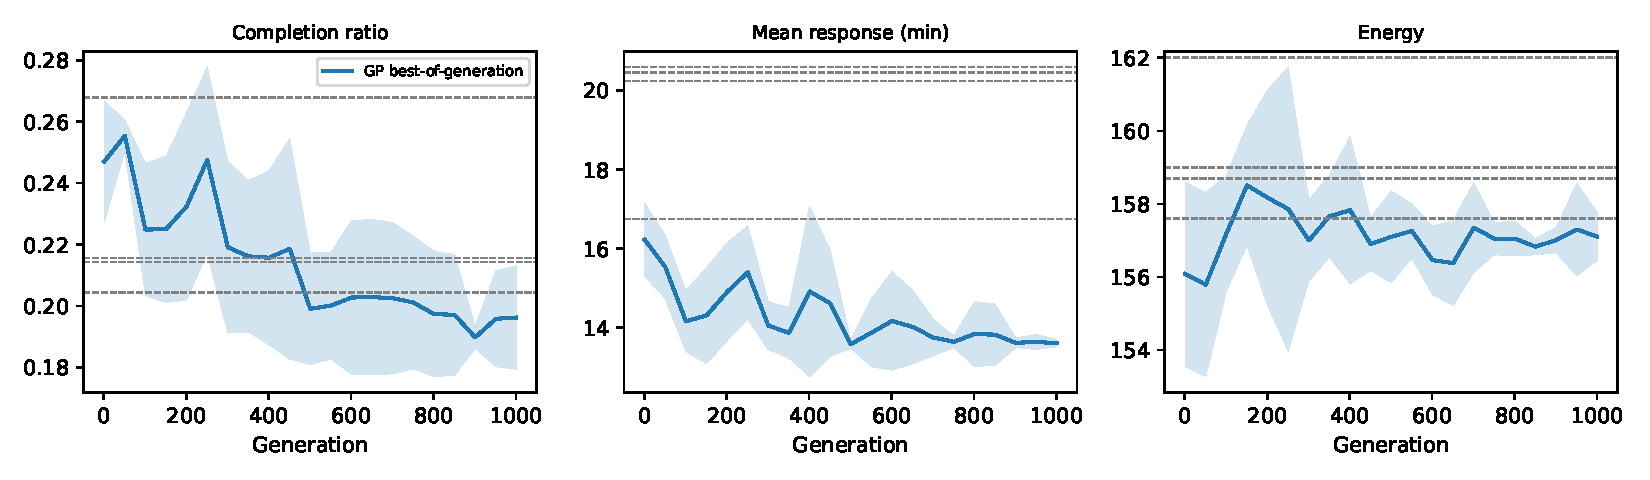
\includegraphics[width=\textwidth]{experiments/results/convergence.pdf}
\caption{Test-world metrics of the best individual of each generation (mean $\pm$
std over 10 seeds). Dashed lines: the four baselines.}
\label{fig:conv}
\end{figure}

Figure~\ref{fig:conv} shows the metrics of the current best individual over
the 1000 generations: $R$ drops from about 16.2 to 14.3\,min within the first 150 generations
(13.6 at the end), while the completion ratio of the best individual goes down
from 0.25 to 0.20.

\section{Parameter Study}
Tables~\ref{tab:depth}--\ref{tab:weights} vary one parameter at a time around
the default configuration (300 generations).

\begin{table}[h]\centering\small\begin{tabular}{lcccc}\toprule
Max.\ depth & $C$ & $R$ (min) & $\mathcal{E}$ & Tree size\\\midrule
2 & 0.202 $\pm$ 0.021 & 13.69 $\pm$ 0.24 & 157.3 $\pm$ 1.2 & 2.0\\
3 & 0.197 $\pm$ 0.019 & 13.64 $\pm$ 0.20 & 156.5 $\pm$ 1.3 & 2.0\\
4 & 0.228 $\pm$ 0.032 & 14.63 $\pm$ 1.16 & 156.1 $\pm$ 1.7 & 7.2\\
5 & 0.222 $\pm$ 0.027 & 13.88 $\pm$ 0.49 & 158.0 $\pm$ 2.0 & 6.2\\
6 & 0.240 $\pm$ 0.019 & 14.51 $\pm$ 0.86 & 157.3 $\pm$ 3.0 & 16.7\\
7 & 0.220 $\pm$ 0.031 & 14.20 $\pm$ 0.85 & 158.7 $\pm$ 2.6 & 11.0\\
\bottomrule
\end{tabular}
\caption{Maximum tree depth.}\label{tab:depth}\end{table}
\begin{table}[h]\centering\small\begin{tabular}{lcccc}\toprule
Population & $C$ & $R$ (min) & $\mathcal{E}$ & Tree size\\\midrule
20 & 0.199 $\pm$ 0.015 & 15.72 $\pm$ 3.42 & 157.8 $\pm$ 1.2 & 1.8\\
50 & 0.212 $\pm$ 0.031 & 14.22 $\pm$ 0.86 & 156.7 $\pm$ 1.4 & 5.8\\
100 & 0.228 $\pm$ 0.032 & 14.63 $\pm$ 1.16 & 156.1 $\pm$ 1.7 & 7.2\\
200 & 0.247 $\pm$ 0.021 & 14.95 $\pm$ 0.88 & 155.7 $\pm$ 2.4 & 12.7\\
400 & 0.250 $\pm$ 0.005 & 14.75 $\pm$ 0.81 & 155.7 $\pm$ 2.8 & 10.6\\
\bottomrule
\end{tabular}
\caption{Population size.}\label{tab:pop}\end{table}
\begin{table}[h]\centering\small\begin{tabular}{lcccc}\toprule
Generations & $C$ & $R$ (min) & $\mathcal{E}$ & Tree size\\\midrule
50 & 0.252 $\pm$ 0.001 & 15.72 $\pm$ 0.37 & 155.6 $\pm$ 0.5 & 13.9\\
100 & 0.241 $\pm$ 0.023 & 14.84 $\pm$ 1.15 & 157.2 $\pm$ 2.7 & 8.8\\
300 & 0.228 $\pm$ 0.032 & 14.63 $\pm$ 1.16 & 156.1 $\pm$ 1.7 & 7.2\\
1000 & 0.197 $\pm$ 0.018 & 13.69 $\pm$ 0.34 & 156.8 $\pm$ 0.2 & 2.4\\
\bottomrule
\end{tabular}
\caption{Number of generations.}\label{tab:gens}\end{table}
\begin{table}[h]\centering\small\begin{tabular}{lcccc}\toprule
Hoist rate & $C$ & $R$ (min) & $\mathcal{E}$ & Tree size\\\midrule
0.0 & 0.232 $\pm$ 0.030 & 14.69 $\pm$ 0.91 & 157.6 $\pm$ 2.9 & 10.9\\
0.05 & 0.228 $\pm$ 0.032 & 14.63 $\pm$ 1.16 & 156.1 $\pm$ 1.7 & 7.2\\
0.2 & 0.196 $\pm$ 0.015 & 13.60 $\pm$ 0.04 & 157.1 $\pm$ 0.5 & 1.2\\
\bottomrule
\end{tabular}
\caption{Hoist rate.}\label{tab:hoist}\end{table}
\begin{table}[h]\centering\small\begin{tabular}{lcccc}\toprule
World switch period (gen.) & $C$ & $R$ (min) & $\mathcal{E}$ & Tree size\\\midrule
1 & 0.208 $\pm$ 0.025 & 13.65 $\pm$ 0.18 & 157.9 $\pm$ 1.4 & 3.5\\
10 & 0.228 $\pm$ 0.032 & 14.63 $\pm$ 1.16 & 156.1 $\pm$ 1.7 & 7.2\\
50 & 0.267 $\pm$ 0.001 & 15.39 $\pm$ 0.72 & 160.8 $\pm$ 3.0 & 15.7\\
$\infty$ & 0.258 $\pm$ 0.007 & 15.81 $\pm$ 0.43 & 157.3 $\pm$ 1.6 & 17.2\\
\bottomrule
\end{tabular}
\caption{Number of generations between world changes ($\infty$: one training world).}\label{tab:switch}\end{table}
\begin{table}[h]\centering\small\begin{tabular}{lcccc}\toprule
Weights $(w_C,w_R,w_E)$ & $C$ & $R$ (min) & $\mathcal{E}$ & Tree size\\\midrule
(0.6, 0.25, 0.15) & 0.228 $\pm$ 0.032 & 14.63 $\pm$ 1.16 & 156.1 $\pm$ 1.7 & 7.2\\
(1.0, 0.0, 0.0) & 0.254 $\pm$ 0.010 & 16.57 $\pm$ 0.65 & 160.3 $\pm$ 2.3 & 13.2\\
(0.34, 0.33, 0.33) & 0.211 $\pm$ 0.041 & 16.87 $\pm$ 1.81 & 156.9 $\pm$ 1.4 & 4.6\\
(0.2, 0.4, 0.4) & 0.203 $\pm$ 0.041 & 17.06 $\pm$ 1.94 & 157.8 $\pm$ 1.0 & 4.2\\
\bottomrule
\end{tabular}
\caption{Fitness weights.}\label{tab:weights}\end{table}

\begin{itemize}
  \item \textbf{Depth} (Table~\ref{tab:depth}). Depths 2--3 give trivial trees
        (size 2) with $C\approx0.20$; depth $\ge4$ gives larger trees and
        $C$ between $0.22$ and $0.24$. Differences between depths 4--7 are within one standard deviation.
  \item \textbf{Population} (Table~\ref{tab:pop}). $C$ grows with population size
        ($0.199$ at 20 to $0.250$ at 400), the clearest monotone trend, with lower
        variance for large populations.
  \item \textbf{Generations} (Table~\ref{tab:gens}). Contrary to expectation, $C$
        \emph{falls} with more generations ($0.252$ at 50, $0.197$ at 1000) while $R$
        falls too, which is the misalignment discussed above.
  \item \textbf{Hoist rate} (Table~\ref{tab:hoist}). 0 and 0.05 are equivalent; 0.2
        collapses the trees to a single node (size 1.2) and loses completion ratio.
  \item \textbf{World switching} (Table~\ref{tab:switch}). Changing the world every
        generation hurts ($C=0.208$); slower switching (50 generations) or a single
        world gives the highest $C$ ($0.267$, $0.258$) but a higher $R$ and larger
        trees. On this dataset we found no sign that a single training world overfits
        more than cycling through worlds.
  \item \textbf{Fitness weights} (Table~\ref{tab:weights}). Weighting completion only
        gives the best $C$ ($0.254$) at the price of a longer $R$ ($16.6$\,min); giving
        more weight to $R$ and $\mathcal{E}$ lowers $C$ to about $0.20$ and does not
        lower $R$.
\end{itemize}

\section{Evolved Rules}
Table~\ref{tab:trees} lists the three best rules of the main runs by test completion ratio.
\begin{table}[h]\centering\small
\begin{enumerate}
\item $C=0.248$, size 15:\\
{\small\texttt{((job.arrivalTime - job.executionTime) - ((MAX(job.disk, job.arrivalTime) * MAX(sat.completedTasks, job.executionTime)) /? MAX(sat.networkBusyUntil, sat.bandwidth)))}}
\item $C=0.191$, size 1:\\
{\small\texttt{job.arrivalTime}}
\item $C=0.191$, size 1:\\
{\small\texttt{job.arrivalTime}}
\end{enumerate}
\caption{Best evolved rules (\texttt{/?} is protected division).}\label{tab:trees}
\end{table}
Many evolved rules reduce to a single terminal, \texttt{job.arrivalTime}, i.e.\
an FCFS-like ordering with the decoder's first-fit satellite choice; the larger
rules combine task execution time and arrival time (a shortest-job-like term)
with satellite load and bandwidth.

\section{Threats to Validity}
\begin{itemize}
  \item One trace, split into consecutive windows: train and test worlds come from the same
        distribution and test worlds are temporally adjacent to training ones.
  \item Worlds are limited to 100 tasks and completion ratios are low
        ($\approx0.2$--$0.3$) because the operational window and energy constraints of the
        decoder reject most pairs; conclusions may change with other loads.
  \item Mean response time over scheduled tasks only (see above); $\mathcal{E}$ varies very little between methods.
  \item The difference between many configurations is of the order of one standard deviation over 10 seeds;
        no significance test was run.
  \item Models are selected with a heuristic (training completion ratio) rather than the fitness itself.
  \item All results use the default selection rule~\eqref{eq:sel-index}. Task-only rules, including
        the FCFS and shortest-job-first baselines and the many evolved single-terminal rules, therefore
        take the first feasible satellite. The earliest-free rule of Section~\ref{sec:ties} has not been
        evaluated (configurations \texttt{tiebreak*} of \texttt{run\_ablation.py}); it changes the
        decoder, so the baselines must be re-scored with it as well.
  \item All results use the population-relative fitness. The fixed-bound fitness of
        Section~\ref{sec:fixed}, designed to remove the misalignment discussed above, has not
        been evaluated yet (configurations \texttt{fixed} and \texttt{fixed+clones+worlds3} of
        \texttt{run\_ablation.py}).
\end{itemize}

\chapter{Conclusions and Future Work}
\label{ch:concl}

We formulated task scheduling in satellite edge computing as a genetic-programming
hyper-heuristic and implemented it as a parallel C++ library. On held-out worlds,
the evolved rules reduce the mean response time of scheduled tasks by about 18\%
with respect to the best hand-written baseline (shortest job first), but the
current fitness does not reward scheduling more tasks: longer training produces
trivial rules and a lower completion ratio. Larger populations and a
completion-only fitness give a higher completion ratio ($0.25$), still below
SJF ($0.27$). The main next step is therefore to redefine the objectives (e.g.\ response time
including unscheduled tasks as penalty) before drawing conclusions on GP versus heuristics.

\section{Future Work}
\label{sec:future}
\begin{itemize}
  \item Multi-tree individuals: separate routing and queuing rules, with elite recombination.
  \item Structured requests: tasks as directed acyclic graphs of dependent services.
  \item Adaptive mutation biased by tree and terminal importance.
  \item Realistic dynamics: NHPP arrivals, moving topology, ISL routing.
  \item Validation on held-out worlds and comparison with the heuristics and ILP of \citet{icdcs_sc}.
\end{itemize}


\bibliographystyle{plainnat}
\bibliography{references}

\end{document}
